\documentclass[12pt,a4paper]{article}
\usepackage[utf8]{inputenc}
\usepackage[english]{babel}
\usepackage{amsmath}
\usepackage{amsfonts}
\usepackage{setspace}
\usepackage{amssymb}
\usepackage{listings}
\usepackage[dvipsnames]{xcolor}
\usepackage{textcomp}
\usepackage[pdftex]{graphicx} 
\usepackage{float}    


\usepackage[left=1in,right=1in,top=1in,bottom=1in]{geometry}
\author{Isaac Evans and Joseph Lynch}
\title{Organon, A Symbolic Constraint Framework And Solver}
\begin{document}

\lstdefinelanguage{Scheme}{
  morekeywords=[1]{define, define-syntax, define-macro, lambda, define-stream, stream-lambda},
  morekeywords=[2]{begin, call-with-current-continuation, call/cc,
    call-with-input-file, call-with-output-file, case, cond,
    do, else, for-each, if,
    let*, let, let-syntax, letrec, letrec-syntax,
    let-values, let*-values,
    and, or, not, delay, force,
    quasiquote, quote, unquote, unquote-splicing,
    map, fold, syntax, syntax-rules, eval, environment, query },
  morekeywords=[3]{import, export},
  alsodigit=!\$\%&*+-./:<=>?@^_~,
  sensitive=true,
  morecomment=[l]{;},
  morecomment=[s]{\#|}{|\#},
  morestring=[b]",
  basicstyle=\small\ttfamily,
  keywordstyle=\bf\ttfamily\color[rgb]{0,.3,.7},
  commentstyle=\color[rgb]{0.133,0.545,0.133},
  stringstyle={\color[rgb]{0.75,0.49,0.07}},
  upquote=true,
  breaklines=true,
  breakatwhitespace=true,
  literate=*{`}{{`}}{1},
  basicstyle=\footnotesize,
}

\lstset{
 language=Scheme
}

\maketitle
\newpage
\tableofcontents
\newpage
\section{Introduction}
Organon is an open source system for expressing and solving complex symbolic constraints between generic entities. It has three main components: 
\begin{enumerate}
\item \texttt{Forms}: Abstract representations of the entities to be constrained
\item \texttt{Constraints}: Functions that symbolically express requirements on the relationships between forms as well as provide information for how a solver can improve upon the constraint's satisfaction.
\item \texttt{Solvers} : Functions which inspect instantiations of forms and manipulate them in an attempt to satisfy a set of objective constraints
\end{enumerate}

Organon is designed to be very generic, which is why it ships with four demonstrations in entirely different domains.  Organon should not constrain the programmers ability to phrase their constraints, it should only give them a framework to express their intentions.

\section{Problem}
The inspiration for Organon was a challenge faced during development work on MIT's entry to the third DARPA Robotics Challenge (DRC). The action authoring system for the DRC needed a way to express constraints between the robot and real-world objects. Ideally, these constraints would be specified symbolically, rather than as fully specified 3D pose offsets. These symbolic constraints could express high-level intents such as ``these hands grasp the ladder rung at a point not so close to the edge that it cannot be reached, but not so close to the center that the hands are more than a shoulder-width apart.'' In our system, once such a constraint function is expressed, it is applicable to any object (for example, stairs instead of  ladder rung) which has the properties required by the constraint function.

Our completed system accommodates this concept of symbolic constraints and is generic enough to allow a host of other constraint expressions that are completely unrelated to 3D concepts.

\section{Organon Library Framework}
The main Organon library provides functions needed to create, manipulate, and constrain forms, as well as two basic implementations of solvers that can iteratively improve form bindings such that constraints become more satisfied.  

\subsection{Forms}
Forms represent a symbolic and straightforward way to represent the world.  Forms have properties, and possibly they have values associated with those properties.  Internally these are represented by \texttt{eq-property} lists so that we can store completely arbitrary properties.  To make working with forms easier, Organon provides a basic typing system that allows the programmer to alias ``types'' to a set of properties. For example, one can declare the form type \texttt{'sphere} to have the properties of \texttt{'center} and \texttt{'radius} with the following code:

\begin{lstlisting}
;; Declare type 'sphere to have a 'center and a 'radius
(declare-form-type 'sphere (list 'center 'radius)) 
\end{lstlisting}

It is important to note that this declaration does not limit the programmer to particular data types, \texttt{'center} can be a vector just as easily as it can be an integer.  Once a type is declared, it is very easy to instantiate forms with all of the properties present in the form type declaration:
\begin{lstlisting}
;; Declare a form 'ball that has all types in the type 'sphere (so 'center and 'radius)
(declare-form 'ball 'sphere) 
\end{lstlisting}

Additionally, Organon provides basic type inheritance, which allows the programmer to specify that a particular form has all the properties associated with another form.   This is useful because it means that people can reuse common property definitions (such as those of a \texttt{3d-object}).  To inform the system about a type inheritance, one can use the declare-type-inherits function to tell the system that one form type should have all properties of another type.  For example, \texttt{sphere}'s are \texttt{3d-object}s made up of vertices, so it would be prudent to give spheres all the properties of 3d-objects:
\begin{lstlisting}

;; Declare that 'sphere inherits all properties of '3d-objects
(declare-type-inherits 'sphere '3d-objects)
\end{lstlisting}

Once a form is declared, it becomes available for the programmer to get and set properties.
\begin{lstlisting}

;; Return the property of form, or #f if there has been no binding
(get-property form property)

;; Set the property of form to be value 
(set-property form property value)
\end{lstlisting}

It is important to note that nothing about Organon's type system limits the programmers ability to set and get arbitrary properties, it just makes it easier for constraints to check that supplied forms have various properties. 

\subsection{Constraints}
Constraints represent an abstraction that allow a programmer to specify how ``satisfied'' he or she is with the state of the world.  Organon presents two types of constraints: basic and compound.  The former expresses constraints over forms, and the latter over other constraints.  These two types ought be sufficient to express the vast majority of real world constraints, but Organon allows the constraint system to be extended if needed.

To create a constraint the programmer must provide two and optionally a third piece of information:
\begin{enumerate}

\item \texttt{operands}: N operands of the constraint, a.k.a ``dependencies'' of that constraint.
\item \texttt{constraint-function}: A function of N arguments that when applied to operands yields a value between 0.0 and 1.0, where 0.0 is completely unsatisfied and 1.0 is completely satisfied.
\item \texttt{(optional) hint-function}:  A function of N arguments that when applied to operands yields a set of potential new bindings for forms that would improve the constraint's satisfaction.  Usually this is only provided for basic forms.

\end{enumerate}
Both basic and compound constraints share the same basic method signature:
\begin{lstlisting}
(make-constraint type operands constraint-function #!optional hint-function)

\end{lstlisting}
For convenience, Organon supplies \texttt{make-compound-constraint} and \texttt{make-basic-constraint} that automatically bind \texttt{type} to the correct entity. One can think of a constraint made in this fashion to be a node in a constraint graph, where edges connect that node to all depended forms or constraints.  Nodes can be ``dirty'' if their dependencies have changed recently, or ``clean'' if their dependencies have not changed since the last evaluation.  Organon keeps track of this information for the programmer and automatically marks nodes as clean and dirty as needed.  For example, when a form binding is changed, that automatically marks basic constraints dependent on that form as dirty so that the next time they are evaluated they will use the new binding of that form.

Internally, make-constraint creates a scheme entity that in addition to storing the clean/dirty state, has the following calling convention:
\begin{lstlisting}
;; Applies constraint-function to operands if the node is ``dirty'', otherwise returns the last known value
(constraint)

;; Applies the hint-function to operands
(constraint 'hint)

;; Returns the operands
(constraint 'children)

;; Applies constraint-function to alternative-arguments
(constraint 'eval alternative-arguments)

;; Returns the type of operands expected ('form or 'constraint)
(constraint 'type) 

;; Forces application of constraint-function to operands regardless of the cleanliness of the constraint.
(constraint 'force)

\end{lstlisting}
The constraint system was architected to be highly generic, and to that end it is very easy to extend with additional types of constraints, e.g. those operating not over forms or other constraints.   All state is maintained in the mit-scheme entity, and the vast majority of state is provided by the closure over the entity.

\subsection{Solvers}

All solvers conform to a common interface by convention. A solver takes as arguments the forms that represent the world state, and the objective constraints from the constraint network that the solver will attempt to satisfy. The solvers operate by use of ``hint'' functions provided by the constraints. The solver can apply a constraint's hint function to improve constraint satisfaction; applying a hint from one constraint, however, might decrease the satisfaction of any number of other constraints. Thus the solver acts as an optimizer, exploring the possible hint applications in the hopes of finding either a perfect satisfaction or the one closest to fully satisfied. Since hints are full-fledged functions, not static recommendations, they may change as the solver runs, since they can depend on the current form bindings. This gives an enormous amount of power to the user to guide solvers into specific solutions.

The solver library also provides substantial utility functions to minimize the code required to write a specific solvers. Most notable is the \texttt{iteratively-score-hints} function, which takes a scoring function and a visualizer function as input and calls each of them after having applied one of the hints given to the world state. We developed two independent solvers for Organon, an iterative exhaustive solver, and an iterative annealing solver.

\subsubsection{Solver 1: Exhaustive}
\begin{lstlisting}
(define (basic-iterative-solver forms objective-constraints)
\end{lstlisting}

The first is an exhaustive solver. Given the objective constraints, it explores the set of all possible subsets of the set of hints attached to the children of those objective constraints. For each subset, it applies the bindings given by the hint function, which triggers all of the constraint values to be recomputed. On each iteration, the exponential solver returns a listing mapping each set to its score (as determined by the provided scoring function, which may take into account weights on the objective constraints).

The exhaustive solver is exponential in complexity. For the set of bindings given by a hint, each binding is applied one at a time, and thus the constraint network updates after each binding. Each iteration of the exhaustive solver takes, in the worst case $O(2^{h}*h*n))$ time, where h is the number of hints and n is the number of constraints. In the typical case where the height of the constraint tree is logarithmic in n, the complexity is $O(2^{h}*h*log(n))$.
\newline

\subsubsection{Solver 2: Annealing}
\begin{lstlisting}
(define (basic-annealing-solver forms objective-constraints iterations)
\end{lstlisting}

The second solver is an ``annealing" solver. This solver takes the set of all hints and then randomly chooses a subset of those hints to apply. The interface to the annealing solver is identical, with an added parameter for the number of iterations to perform. Each iteration is $O(h * log(n))$ in typical complexity and $O(h*n)$ in worst case complexity, where h is the number of hints generated and n is the size of the constraint graph.   The intuition behind this solver is that there is no way to know which combination of hints lead to a solution state, but the hints recompute every iteration, so we can always fix ourselves later by taking a different set of hints.  The annealing comes from decreasing this probability with time, which guarantees that after a certain amount of time we will settle at some state, even if that state is not globally optimal.  

The annealing solver does not provably find a solution state, it instead relies on the hint functions to return good hints that move the state of the system quickly towards a solution.  It is important to note that the hints are local as generally there is no knowledge of global state accessible to constraints.  While this may make many computer scientists and mathematicians nervous because we cannot guarantee or prove much, in the real world this solver is often sufficient to find goal states and does so very quickly.  In particular, this solver is useful because while it may not return a globally optimal solution, it does return a locally optimal solution, and those tend to be sufficient.  For example, we implemented graph coloring with the annealing solver and while it can theoretically not find a solution, it usually quickly finds a decent solution and in all cases we tested it on, it found a correct coloring.

\section{Example Uses of Organon}

As the purpose of Organon was to provide a general framework to reason about constraints, we present four demonstrations of its capabilities in three different problem domains: engineering, economics, and mathematics.

For visualization purposes, we wrote opengl-streamer.scm, which makes a socket connection to a multithreaded C++ server, which parses the incoming message and converts it to OpenGL objects. The message protocol supports OpenGL primitives (box, sphere, cylinder) as well as raw vertex lists. This allows us to visualize constraint application in real time. 

We also wrote a simplified REPL for loading and running demo programs.
\subsection{Ladder}
The ladder demo (ladder.scm) defines two constraints, \texttt{hands-far-away} and \texttt{hands-end-of-rung}. These constraints provide hints which move the hands incrementally farther away from each other and incrementally towards the end of the rung, respectively.  
\begin{lstlisting}
(define hands-far-away
  (make-basic-constraint
    '(left-hand right-hand desired-distance)
	;; lots of calls in between to extract the 3D components of interest
    (make-binding-list
      (make-binding
      left-hand
      (list 'frame (make-frame (add-vector left-hand-vector left-hand-inverted)
                               left-hand-quat)))
	;; right hand is symmetric, omitted for brevity
\end{lstlisting}

Finally, the demo uses the compound constraint \texttt{hands-on-ladder} to wrap both of the subconstraints. The satisfaction of \texttt{hands-on-ladder} is the average of the satisfactions of the subconstraints.
\begin{lstlisting}

(define hands-on-ladder
  (make-compound-constraint
    (list hands-far-away hands-end-of-rung)
	...
\end{lstlisting}

When run with the exponential solver, the ladder demo rapidly explores the space of hinted hand positions and finally settles on a final binding that puts the hands on opposite ends of the rung, as intended.
<image>

\subsection{Big Bang}

This demo (big-bang.scm) defines one hundred "star" forms, each of which have a center and radius. The forms begin at the origin, and there is a single basic constraint: the universe, which calculates center of mass of the universe and hints each star to move slightly away from that center of mass. 
\begin{lstlisting}

(define (universe-constraint d . forms)
    ...
    (define (score-single form)
      (let* ((pos (get-property form 'center))
             (dis (distance center-of-mass pos)))
        (min 1.0 (/ dis (get-value d)))))
    (/ (apply + (map score-single forms)) (length forms))))
\end{lstlisting}

The annealing solver is used to run this demo; obviously, the exponential solver would have bad time with a $2^{100}$ search space. On each iteration, the annealing solver randomly moves the ``star'' forms further away. When the network-visualizer function is passed to the solver, the resulting universe expansion can be visualized in OpenGL.
<image>

\subsection{Laffer Curve}

This demo (laffer.scm) defines one hundred ``tax-payer'' forms, each of which have plausible weekly wage rates, maximum number of hours they are willing to work, and their liberalness (how willing they are to work given taxation).  The forms are bound by a single constraint, the laffer constraint. This expresses that the government attempts to maximize tax revenue from taxpayers who work fewer hours based on the given tax rate:
\begin{lstlisting}

;; constraint returns a value in range [0.0, 1.0] is (revenue at tax-rate /
;; maximum possible revenue)
(define (laffer-constraint tax-rate . taxpayers)
  (/ (apply + (map (lambda (ith-taxpayer)
                     ;; (1 - t^l) * maximum hours = number of hours worked
                     ;; * hourly wages = output of this person
                     ;; * tax rate = taxes collected by the government
                     (* (- 1.0 (expt (get-value tax-rate) (get-property ith-taxpayer 'liberalness)))
                        (get-property ith-taxpayer 'max-hours-worked)
                        (get-property ith-taxpayer 'hourly-wage)
                        (get-value tax-rate)))
                   taxpayers))
     (apply + (map (lambda (ith-taxpayer)
                     ;; Maximum possible output of the economy
                     (* (get-property ith-taxpayer 'max-hours-worked)
                        (get-property ith-taxpayer 'hourly-wage))) taxpayers))))
\end{lstlisting}

This constraint hints that taxes should decrease by 1 percent, and since taxation starts at 100\%, this has the effect of causing the solver to explore the entire taxation rate from 100\% down to 0\%.  The annealing solver is again used, and we can use the outputs of the solver to construct the laffer curve as seen in Figure ~\ref{fig:laffer}

\begin{figure}[H]
\caption{Simulated Laffer Curve}
\centering
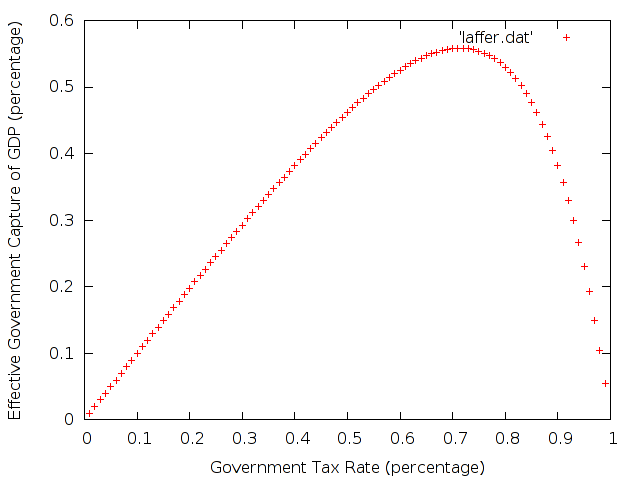
\includegraphics[scale=.5]{../demos/laffer.png}
\label{fig:laffer}
\end{figure}

Apparently, with our simplistic model, an effective government tax rate of ~71\% would mean maximum government revenue.  Note that this is not the same as maximizing societal welfare or happiness, and an interesting addition would be to add another constraint that optimizes for that.

\subsection{Graph Coloring}

This demo (hard-coloring.scm) defines node forms that can have a color and then constraints for each edge between two nodes such that we construct the classic Peterson Graph seen in Figure \ref{fig:Peterson}.  The annealing solver is then used to find a potential coloring, often completing within 100-120 iterations.
\begin{figure}[H]
\caption{Peterson Graph with Valid 3-Coloring}
\centering
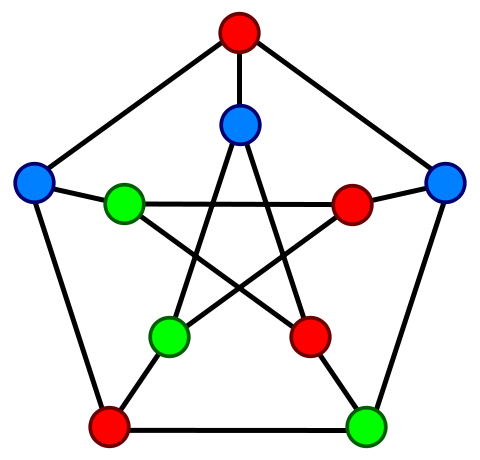
\includegraphics[scale=.5]{peterson.png}
\label{fig:Peterson}
\end{figure}

All of the graph coloring demos use the same basic constraint and hint defined on any two nodes
\begin{lstlisting}
;; Neighboring Nodes must be colored differently
(define (Node-constraint x y)
  (if (not (eq? (get-property x 'color) (get-property y 'color)))
    1.0
    0.0))

;; If two nodes are different colors, with high probability stay the same
;; otherwise switch one of them to another viable coloring
;;
;; If two nodes are the same color, change one of them to be a different
;; color
(define (Node-hint x y)
  (let ((x-color (get-property x 'color))
        (y-color (get-property y 'color)))
    (if (null? x-color)
      (make-binding-list
        (make-binding x (list 'color (car (get-value 'colors)))))
      (cond
        ;; Different colors already? with high probability hint at nothing
        ((and (eq? x-color y-color) (> (random 5) 2))
         (make-binding-list))
        (else
          ;; Hint at a randomly chosen alternative for y
          (make-binding-list
            (random-choice
              (map (lambda (color)
                     (make-binding y (list 'color color)))
                   (filter (lambda (z) (not (eq? z x-color))) (get-value 'colors))))))))))
\end{lstlisting}

This relies on local swaps with probabilistic transitions to color the graph.  This is not provably correct, but in all of the demonstration graphs provided, it works very quickly (and finds an acceptable answer within 1 or 2 iterations). While this isn't particularly useful for proving that a graph is n-colorable, it is very useful for situations where coloring need only be approximate and you know the number of available colors, such as register allocation within a compiler.

\section{Future Work \& Conclusions:}
Organon presents a powerful and generic way for programmers to specify constraints in real world problems as well as easily build solvers to explore those constraint domains.  It relies on numerous concepts learned in 6.945 such as generic operations, propagators, and the idea that flexibility is sometimes more important than correctness.  Although we cannot prove its usefulness, and we cannot prove its correctness, if there is one thing that 6.945 teaches, it is that nobody really can.  Organon focuses on being generally useful, on allowing the end user to use the system in the ways that they see fit.

Organon's provided solvers are sufficient for many problems, but the most difficult constraint optimization and satisfaction problems require techniques far more advanced than those presented here.  An interesting avenue of research would therefore be to explore additional optimization techniques such as complete simulated annealing with variable probabilistic transitions, hill climbing, particle swarm optimization, et. al.

The main disadvantage to Organon's powerful constraint system is that the constraint functions--though often simple in concept--are not readable except to a reasonably sophisticated expert. In the future, we might build a dedicated constraint language to eliminate much of the verbosity of that is currently involved in ensuring that the forms passed to a constraint function are of the appropriate type and extracting and manipulating their properties.

All code is available at https://github.com/jolynch/organon.

\appendix
\section{Appendix A - Library}\label{App:AppendixA}
\subsection{forms.scm}
\lstinputlisting{../lib/constraints.scm}
\subsection{constraints.scm}
\lstinputlisting{../lib/forms.scm}
\subsection{solver.scm}
\lstinputlisting{../lib/solver.scm}
\subsection{util.scm}
\lstinputlisting{../lib/util.scm}
\subsection{opengl-stream.scm}
\lstinputlisting{../lib/util.scm}
\newpage

\section{Appendix B - Demos}\label{App:AppendixB}
\subsection{ladder.scm}
\lstinputlisting{../demos/ladder.scm}
\subsection{big-bang.scm}
\lstinputlisting{../demos/big-bang.scm}
\subsection{laffer.scm}
\lstinputlisting{../demos/laffer.scm}
\subsection{node-coloring.scm}
\lstinputlisting{../demos/node-coloring.scm}
\subsection{harder-coloring.scm}
\lstinputlisting{../demos/harder-coloring.scm}
\end{document}